
%% bare_conf.tex
%% V1.3
%% 2007/01/11
%% by Michael Shell
%% See:
%% http://www.michaelshell.org/
%% for current contact information.
%%
%% This is a skeleton file demonstrating the use of IEEEtran.cls
%% (requires IEEEtran.cls version 1.7 or later) with an IEEE conference paper.
%%
%% Support sites:
%% http://www.michaelshell.org/tex/ieeetran/
%% http://www.ctan.org/tex-archive/macros/latex/contrib/IEEEtran/
%% and
%% http://www.ieee.org/

%%*************************************************************************
%% Legal Notice:
%% This code is offered as-is without any warranty either expressed or
%% implied; without even the implied warranty of MERCHANTABILITY or
%% FITNESS FOR A PARTICULAR PURPOSE! 
%% User assumes all risk.
%% In no event shall IEEE or any contributor to this code be liable for
%% any damages or losses, including, but not limited to, incidental,
%% consequential, or any other damages, resulting from the use or misuse
%% of any information contained here.
%%
%% All comments are the opinions of their respective authors and are not
%% necessarily endorsed by the IEEE.
%%
%% This work is distributed under the LaTeX Project Public License (LPPL)
%% ( http://www.latex-project.org/ ) version 1.3, and may be freely used,
%% distributed and modified. A copy of the LPPL, version 1.3, is included
%% in the base LaTeX documentation of all distributions of LaTeX released
%% 2003/12/01 or later.
%% Retain all contribution notices and credits.
%% ** Modified files should be clearly indicated as such, including  **
%% ** renaming them and changing author support contact information. **
%%
%% File list of work: IEEEtran.cls, IEEEtran_HOWTO.pdf, bare_adv.tex,
%%                    bare_conf.tex, bare_jrnl.tex, bare_jrnl_compsoc.tex
%%*************************************************************************

% *** Authors should verify (and, if needed, correct) their LaTeX system  ***
% *** with the testflow diagnostic prior to trusting their LaTeX platform ***
% *** with production work. IEEE's font choices can trigger bugs that do  ***
% *** not appear when using other class files.                            ***
% The testflow support page is at:
% http://www.michaelshell.org/tex/testflow/



% Note that the a4paper option is mainly intended so that authors in
% countries using A4 can easily print to A4 and see how their papers will
% look in print - the typesetting of the document will not typically be
% affected with changes in paper size (but the bottom and side margins will).
% Use the testflow package mentioned above to verify correct handling of
% both paper sizes by the user's LaTeX system.
%
% Also note that the "draftcls" or "draftclsnofoot", not "draft", option
% should be used if it is desired that the figures are to be displayed in
% draft mode.
%
%&latex
\documentclass[10pt, conference, compsocconf]{IEEEtran}
% Add the compsocconf option for Computer Society conferences.
%
% If IEEEtran.cls has not been installed into the LaTeX system files,
% manually specify the path to it like:
% \documentclass[conference]{../sty/IEEEtran}





% Some very useful LaTeX packages include:
% (uncomment the ones you want to load)


% *** MISC UTILITY PACKAGES ***
%
%\usepackage{ifpdf}
% Heiko Oberdiek's ifpdf.sty is very useful if you need conditional
% compilation based on whether the output is pdf or dvi.
% usage:
% \ifpdf
%   % pdf code
% \else
%   % dvi code
% \fi
% The latest version of ifpdf.sty can be obtained from:
% http://www.ctan.org/tex-archive/macros/latex/contrib/oberdiek/
% Also, note that IEEEtran.cls V1.7 and later provides a builtin
% \ifCLASSINFOpdf conditional that works the same way.
% When switching from latex to pdflatex and vice-versa, the compiler may
% have to be run twice to clear warning/error messages.






% *** CITATION PACKAGES ***
%
\usepackage{cite}
% cite.sty was written by Donald Arseneau
% V1.6 and later of IEEEtran pre-defines the format of the cite.sty package
% \cite{} output to follow that of IEEE. Loading the cite package will
% result in citation numbers being automatically sorted and properly
% "compressed/ranged". e.g., [1], [9], [2], [7], [5], [6] without using
% cite.sty will become [1], [2], [5]--[7], [9] using cite.sty. cite.sty's
% \cite will automatically add leading space, if needed. Use cite.sty's
% noadjust option (cite.sty V3.8 and later) if you want to turn this off.
% cite.sty is already installed on most LaTeX systems. Be sure and use
% version 4.0 (2003-05-27) and later if using hyperref.sty. cite.sty does
% not currently provide for hyperlinked citations.
% The latest version can be obtained at:
% http://www.ctan.org/tex-archive/macros/latex/contrib/cite/
% The documentation is contained in the cite.sty file itself.



% *** CITATION PACKAGES ***
%
%\ifCLASSOPTIONcompsoc
%  % IEEE Computer Society needs nocompress option
%  % requires cite.sty v4.0 or later (November 2003)
%  \usepackage[nocompress]{cite}
%\else
%  % normal IEEE
%  \usepackage{cite}
%\fi
%

% *** GRAPHICS RELATED PACKAGES ***
%
\ifCLASSINFOpdf
  \usepackage[pdftex]{graphicx}
  % declare the path(s) where your graphic files are
  % \graphicspath{{../pdf/}{../jpeg/}}
  % and their extensions so you won't have to specify these with
  % every instance of \includegraphics
  % \DeclareGraphicsExtensions{.pdf,.jpeg,.png}
\else
  % or other class option (dvipsone, dvipdf, if not using dvips). graphicx
  % will default to the driver specified in the system graphics.cfg if no
  % driver is specified.
%\usepackage[dvipdfmx]{graphicx} %for Japanese
\usepackage{graphicx} % for  English
  % declare the path(s) where your graphic files are
  % \graphicspath{{../eps/}}
  % and their extensions so you won't have to specify these with
  % every instance of \includegraphics
  % \DeclareGraphicsExtensions{.eps}
\fi
% graphicx was written by David Carlisle and Sebastian Rahtz. It is
% required if you want graphics, photos, etc. graphicx.sty is already
% installed on most LaTeX systems. The latest version and documentation can
% be obtained at: 
% http://www.ctan.org/tex-archive/macros/latex/required/graphics/
% Another good source of documentation is "Using Imported Graphics in
% LaTeX2e" by Keith Reckdahl which can be found as epslatex.ps or
% epslatex.pdf at: http://www.ctan.org/tex-archive/info/
%
% latex, and pdflatex in dvi mode, support graphics in encapsulated
% postscript (.eps) format. pdflatex in pdf mode supports graphics
% in .pdf, .jpeg, .png and .mps (metapost) formats. Users should ensure
% that all non-photo figures use a vector format (.eps, .pdf, .mps) and
% not a bitmapped formats (.jpeg, .png). IEEE frowns on bitmapped formats
% which can result in "jaggedy"/blurry rendering of lines and letters as
% well as large increases in file sizes.
%
% You can find documentation about the pdfTeX application at:
% http://www.tug.org/applications/pdftex





% *** MATH PACKAGES ***
%
%\usepackage[cmex10]{amsmath}
% A popular package from the American Mathematical Society that provides
% many useful and powerful commands for dealing with mathematics. If using
% it, be sure to load this package with the cmex10 option to ensure that
% only type 1 fonts will utilized at all point sizes. Without this option,
% it is possible that some math symbols, particularly those within
% footnotes, will be rendered in bitmap form which will result in a
% document that can not be IEEE Xplore compliant!
%
% Also, note that the amsmath package sets \interdisplaylinepenalty to 10000
% thus preventing page breaks from occurring within multiline equations. Use:
%\interdisplaylinepenalty=2500
% after loading amsmath to restore such page breaks as IEEEtran.cls normally
% does. amsmath.sty is already installed on most LaTeX systems. The latest
% version and documentation can be obtained at:
% http://www.ctan.org/tex-archive/macros/latex/required/amslatex/math/





% *** SPECIALIZED LIST PACKAGES ***
%
%\usepackage{algorithmic}
% algorithmic.sty was written by Peter Williams and Rogerio Brito.
% This package provides an algorithmic environment fo describing algorithms.
% You can use the algorithmic environment in-text or within a figure
% environment to provide for a floating algorithm. Do NOT use the algorithm
% floating environment provided by algorithm.sty (by the same authors) or
% algorithm2e.sty (by Christophe Fiorio) as IEEE does not use dedicated
% algorithm float types and packages that provide these will not provide
% correct IEEE style captions. The latest version and documentation of
% algorithmic.sty can be obtained at:
% http://www.ctan.org/tex-archive/macros/latex/contrib/algorithms/
% There is also a support site at:
% http://algorithms.berlios.de/index.html
% Also of interest may be the (relatively newer and more customizable)
% algorithmicx.sty package by Szasz Janos:
% http://www.ctan.org/tex-archive/macros/latex/contrib/algorithmicx/




% *** ALIGNMENT PACKAGES ***
%
%\usepackage{array}
% Frank Mittelbach's and David Carlisle's array.sty patches and improves
% the standard LaTeX2e array and tabular environments to provide better
% appearance and additional user controls. As the default LaTeX2e table
% generation code is lacking to the point of almost being broken with
% respect to the quality of the end results, all users are strongly
% advised to use an enhanced (at the very least that provided by array.sty)
% set of table tools. array.sty is already installed on most systems. The
% latest version and documentation can be obtained at:
% http://www.ctan.org/tex-archive/macros/latex/required/tools/


%\usepackage{mdwmath}
%\usepackage{mdwtab}
% Also highly recommended is Mark Wooding's extremely powerful MDW tools,
% especially mdwmath.sty and mdwtab.sty which are used to format equations
% and tables, respectively. The MDWtools set is already installed on most
% LaTeX systems. The lastest version and documentation is available at:
% http://www.ctan.org/tex-archive/macros/latex/contrib/mdwtools/


% IEEEtran contains the IEEEeqnarray family of commands that can be used to
% generate multiline equations as well as matrices, tables, etc., of high
% quality.


%\usepackage{eqparbox}
% Also of notable interest is Scott Pakin's eqparbox package for creating
% (automatically sized) equal width boxes - aka "natural width parboxes".
% Available at:
% http://www.ctan.org/tex-archive/macros/latex/contrib/eqparbox/





% *** SUBFIGURE PACKAGES ***
%\usepackage[tight,footnotesize]{subfigure}
% subfigure.sty was written by Steven Douglas Cochran. This package makes it
% easy to put subfigures in your figures. e.g., "Figure 1a and 1b". For IEEE
% work, it is a good idea to load it with the tight package option to reduce
% the amount of white space around the subfigures. subfigure.sty is already
% installed on most LaTeX systems. The latest version and documentation can
% be obtained at:
% http://www.ctan.org/tex-archive/obsolete/macros/latex/contrib/subfigure/
% subfigure.sty has been superceeded by subfig.sty.



%\usepackage[caption=false]{caption}
%\usepackage[font=footnotesize]{subfig}
% subfig.sty, also written by Steven Douglas Cochran, is the modern
% replacement for subfigure.sty. However, subfig.sty requires and
% automatically loads Axel Sommerfeldt's caption.sty which will override
% IEEEtran.cls handling of captions and this will result in nonIEEE style
% figure/table captions. To prevent this problem, be sure and preload
% caption.sty with its "caption=false" package option. This is will preserve
% IEEEtran.cls handing of captions. Version 1.3 (2005/06/28) and later 
% (recommended due to many improvements over 1.2) of subfig.sty supports
% the caption=false option directly:
%\usepackage[caption=false,font=footnotesize]{subfig}
%
% The latest version and documentation can be obtained at:
% http://www.ctan.org/tex-archive/macros/latex/contrib/subfig/
% The latest version and documentation of caption.sty can be obtained at:
% http://www.ctan.org/tex-archive/macros/latex/contrib/caption/




% *** FLOAT PACKAGES ***
%
%\usepackage{fixltx2e}
% fixltx2e, the successor to the earlier fix2col.sty, was written by
% Frank Mittelbach and David Carlisle. This package corrects a few problems
% in the LaTeX2e kernel, the most notable of which is that in current
% LaTeX2e releases, the ordering of single and double column floats is not
% guaranteed to be preserved. Thus, an unpatched LaTeX2e can allow a
% single column figure to be placed prior to an earlier double column
% figure. The latest version and documentation can be found at:
% http://www.ctan.org/tex-archive/macros/latex/base/



%\usepackage{stfloats}
% stfloats.sty was written by Sigitas Tolusis. This package gives LaTeX2e
% the ability to do double column floats at the bottom of the page as well
% as the top. (e.g., "\begin{figure*}[!b]" is not normally possible in
% LaTeX2e). It also provides a command:
%\fnbelowfloat
% to enable the placement of footnotes below bottom floats (the standard
% LaTeX2e kernel puts them above bottom floats). This is an invasive package
% which rewrites many portions of the LaTeX2e float routines. It may not work
% with other packages that modify the LaTeX2e float routines. The latest
% version and documentation can be obtained at:
% http://www.ctan.org/tex-archive/macros/latex/contrib/sttools/
% Documentation is contained in the stfloats.sty comments as well as in the
% presfull.pdf file. Do not use the stfloats baselinefloat ability as IEEE
% does not allow \baselineskip to stretch. Authors submitting work to the
% IEEE should note that IEEE rarely uses double column equations and
% that authors should try to avoid such use. Do not be tempted to use the
% cuted.sty or midfloat.sty packages (also by Sigitas Tolusis) as IEEE does
% not format its papers in such ways.





% *** PDF, URL AND HYPERLINK PACKAGES ***
%
%\usepackage{url}
% url.sty was written by Donald Arseneau. It provides better support for
% handling and breaking URLs. url.sty is already installed on most LaTeX
% systems. The latest version can be obtained at:
% http://www.ctan.org/tex-archive/macros/latex/contrib/misc/
% Read the url.sty source comments for usage information. Basically,
% \url{my_url_here}.





% *** Do not adjust lengths that control margins, column widths, etc. ***
% *** Do not use packages that alter fonts (such as pslatex).         ***
% There should be no need to do such things with IEEEtran.cls V1.6 and later.
% (Unless specifically asked to do so by the journal or conference you plan
% to submit to, of course. )


% correct bad hyphenation here
\hyphenation{op-tical net-works semi-conduc-tor}


\bibliographystyle{plain}
\usepackage{url}
%\usepackage{hyperref}
\usepackage{float}
\usepackage{color}
\usepackage{threeparttable}%テーブル内に角柱
\usepackage{hyperref}
%\usepackage{hyperref}
\usepackage{ascmac}%テーブル内に角柱
\usepackage{subfig}


\newcommand{\rr}[1]{\textcolor{red}{#1}}% 赤い文字
\newcommand{\bb}[1]{\textcolor{blue}{#1}}% 青い文字
\newcommand{\cc}[1]{\textcolor{magenta}{#1}}% 青い文字
\newcommand{\mr}[1]{\textcolor{red}{\bf#1}}% 赤い文字強調
\newcommand{\mb}[1]{\textcolor{blue}{\bf#1}}% 青い文字強調
\newcommand{\tr}[1]{\textcolor{red}{\textbf{#1}}}  %% red text
\newcommand{\myurl}[1]{\href{#1}{#1}} %need \usepackage[dvipdfmx]{hyperref}

\begin{document}
%
% paper title
% can use linebreaks \\ within to get better formatting as desired
\title{Visualizing Shiga prefecture using RESAS: cloud-based analysis system with government open big data}


% author names and affiliations
% use a multiple column layout for up to two different
% affiliations

\author{
\IEEEauthorblockN{Jongchan Lee}
\IEEEauthorblockA{
The Center for Data Science\\Education and Research
\\Shiga University\\Hikone, Japan\\j-lee@biwako.shiga-u.ac.jp}
\\
\IEEEauthorblockN{Takuma Tanaka}
\IEEEauthorblockA{
Faculty of Data Science
\\Shiga University\\Hikone, Japan\\takuma-tanaka@biwako.shiga-u.ac.jp}
\and
\IEEEauthorblockN{Tetsuto Himeno}
\IEEEauthorblockA{
Faculty of Data Science
\\Shiga University\\Hikone, Japan\\tetsuto-himeno@biwako.shiga-u.ac.jp}
\\
\\
\IEEEauthorblockN{Akimichi Takemura}
\IEEEauthorblockA{
Faculty of Data Science
\\Shiga University\\Hikone, Japan\\a-takemura@biwako.shiga-u.ac.jp}
\and
\IEEEauthorblockN{Shohei Shimizu}
\IEEEauthorblockA{
Faculty of Data Science
\\Shiga University\\Hikone, Japan\\shohei-shimizu@biwako.shiga-u.ac.jp}
}

% conference papers do not typically use \thanks and this command
% is locked out in conference mode. If really needed, such as for
% the acknowledgment of grants, issue a \IEEEoverridecommandlockouts
% after \documentclass

% for over three affiliations, or if they all won't fit within the width
% of the page, use this alternative format:
% 
%\author{\IEEEauthorblockN{Michael Shell\IEEEauthorrefmark{1},
%Homer Simpson\IEEEauthorrefmark{2},
%James Kirk\IEEEauthorrefmark{3}, 
%Montgomery Scott\IEEEauthorrefmark{3} and
%Eldon Tyrell\IEEEauthorrefmark{4}}
%\IEEEauthorblockA{\IEEEauthorrefmark{1}School of Electrical and Computer Engineering\\
%Georgia Institute of Technology,
%Atlanta, Georgia 30332--0250\\ Email: see http://www.michaelshell.org/contact.html}
%\IEEEauthorblockA{\IEEEauthorrefmark{2}Twentieth Century Fox, Springfield, USA\\
%Email: homer@thesimpsons.com}
%\IEEEauthorblockA{\IEEEauthorrefmark{3}Starfleet Academy, San Francisco, California 96678-2391\\
%Telephone: (800) 555--1212, Fax: (888) 555--1212}
%\IEEEauthorblockA{\IEEEauthorrefmark{4}Tyrell Inc., 123 Replicant Street, Los Angeles, California 90210--4321}}




% use for special paper notices
%\IEEEspecialpapernotice{(Invited Paper)}




% make the title area
\maketitle


\begin{abstract}
RESAS (Regional Economy Society Analyzing System) is 
a cloud based visualization system for Japanese government open data and is useful for regional policy making and business.
In this paper, we discuss two kinds of problems in Shiga prefecture by using 
RESAS and Japanese government open data.
We first consider population trend and movement of Shiga prefecture
%We show the overall population change 
and find other prefectures that are highly related to Shiga's population movement. We take a closer look at the population change of the age of 20s.
Then we present the topic of tourism in Shiga prefecture.
We discuss strength and weakness of Shiga in terms of tourism resource, show statistics
of domestic and international tourism, and propose tourism strategies appropriate for the local government of Shiga. 
\end{abstract}

\begin{IEEEkeywords}
RESAS; big data; government open data; public data; visualization;
\end{IEEEkeywords}


% For peer review papers, you can put extra information on the cover
% page as needed:
% \ifCLASSOPTIONpeerreview
% \begin{center} \bfseries EDICS Category: 3-BBND \end{center}
% \fi
%
% For peerreview papers, this IEEEtran command inserts a page break and
% creates the second title. It will be ignored for other modes.
\IEEEpeerreviewmaketitle



%--------------------------------------------------------------------------------

\section{Introduction}

The demand for effective use of government open data (GOD) has increased in recent years.
Most countries have their own official organization which conduct survey and provide GOD, such as population census, industrial report, employee report and so on \cite{climate,god1, uscensus}.
Moreover, it is not difficult to get intergovernmental comparable statistics on a wide number of subjects. For example, OECD (Organisation for Economic Co-operation and Development) statistics are available in several forms of files in the statistics portal website of OECD\cite{oecd}. 


The Japanese government also has the Statistics Bureau which
conducts fundamental censuses and statistical surveys, and other relevant ministries produce statistics for their own policy purposes. 
The ``Portal Site of Official Statistics of Japan (e-Stat)", established in 2008, provides a one-stop online service for obtaining statistical information published by ministries on the internet and helps users to download official statistics with convenient features such as retrieving data by prefecture and municipality\cite{jpcensus, estat}.

On the other hand, viewed from the point of data analysis, data visualization has become more and more important,
because it is a quick and easy way to convey concepts in an effective manner, to translate big data into practical knowledge \cite{bigdata,bigdata1, bigdata3, bigdata4, visual, visual1}. 
Hence data analysis usually starts with drawing charts or graphs to visualize relations of complex data. 
However, data visualization is not a simple process at all. 
For example, one who already has GOD, would have difficulty to draw a time series graph to see the past 10 years' population inflow into a certain prefecture. Sometimes it is time consuming to determine what types of graph are suitable, 
and requires good understanding of statistical software skills about R, SAS, SPSS, Excel etc.
For this reason, from April 2015, 
the Cabinet Secretariat and the Ministry of Economy, Trade and Industry,  
launched RESAS (Regional Economy Society Analyzing System). It also has become one of the world's largest visualization systems for Japanese GOD.

The objective of RESAS is to assist whoever wants to analyze public data easily\cite{resas} and eventually provide valuable insights to local government decision-makers or civilians through quick data visualization such as tile plot, path plot and so on. 
It is possible to draw the same graphs by using other software such as R, SAS, SPSS and Excel as well. However, RESAS has an advantage that it does not require collecting and importing data because it is implemented on the website. In addition, it is very easy to learn for beginners with little statistical knowledge. 

This paper describes a part of our collaborative project with the local government of Shiga prefecture. 
The project was planned to find out the existing regional social problems mainly related to population and economy. We only used Japanese government open data and RESAS to conduct the project.

In this paper, we focused only on topics of population and tourism issues to discuss the Shiga's current regional economy situation, since these issues are thought to be considerable factors 
which affect the regional economy.
Thus, the purpose of this paper is to clarify Shiga's strength or weakness in terms of  population and tourism by comparing Shiga to other prefectures under the similar situation of Shiga.
For the population analysis, we first start with the overall population situation in Japan, and pay special attention to the population change of age of 20s.
For the tourism analysis, we also start from the overall tourism situation and then compare Shiga to two prefectures.
Secondary purpose of this paper is to introduce the useful 
visualization functions of RESAS.



The organization of this paper is as follows. 
In section \ref{sec:pop}, we will start by presenting overall population situations followed by comparison of Shiga's 
population movement
among the other major cities in Japan.
In Section \ref{sec:tour}, we will discuss strength and weakness of Shiga in terms of tourism resources, and propose tourism strategies appropriate for government of Shiga. 
We end the paper with some discussions on further study in Section \ref{sec:discuss}.


%----------------------------------------------------------------
\section{The general population situation of Shiga}\label{sec:pop}
In this section, we discuss overall population trend and population movement of Shiga. 
In particular, we pay attention to the population change of the age of 20s by comparing Otsu city to several cities in Japan.

\subsection{Population decline}
According to Japanese Ministry of Internal Affairs and Communications Japanese population reached the peak of 128 million people in 2008.
Shiga is one of the few prefectures at which population was still increasing. Its population is estimated to peak at 1.4 million people in 2015. However, after reaching this maximum, it would decline slightly to 1.3 million in 2040 (Fig.~\ref{fig1}). 

Another RESAS plot, such as Fig.~\ref{fig2}, helps more comprehensive and easier understanding of factor causing the population change in Shiga. 
During the periods from 1964 to 1967 (forth quadrant), natural increase was the primary factor behind population growth, while both natural and migratory increase are the contributor to population growth from 1970s to 2010s. It is moving toward the lower-left direction of Fig.~\ref{fig2}, that means Shiga would fall in population decline in a few years. 

\begin{figure}[!t]
\begin{center}
%    %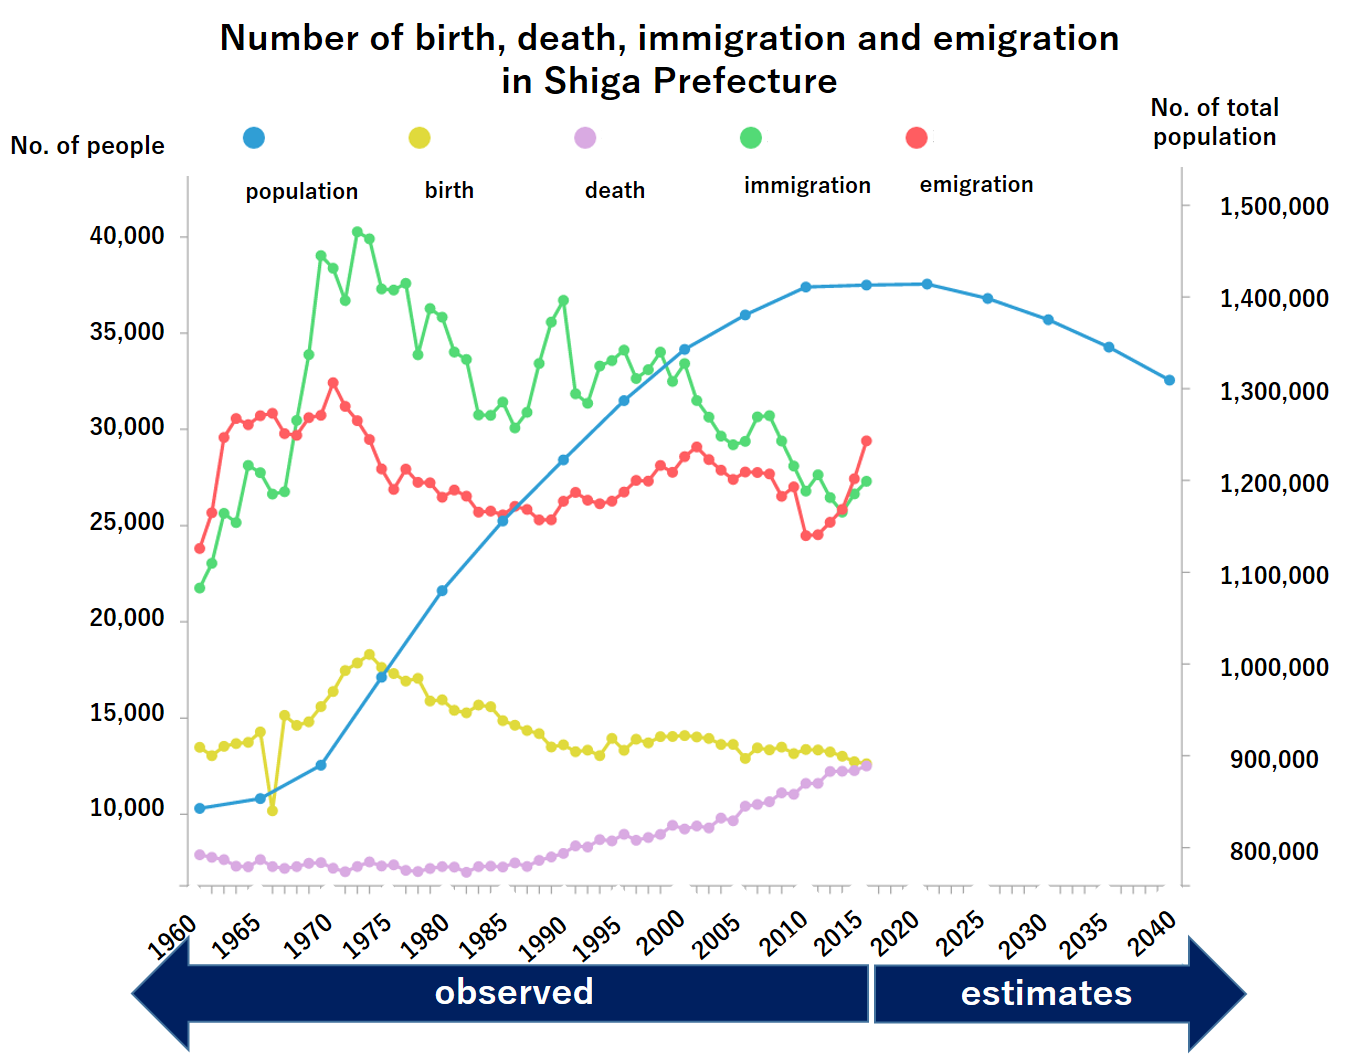
\includegraphics[width= 7cm]{fig/fig1_1.PNG}
\caption{RESAS trend lines of population (blue), births (yellow), deaths (purple), immigration (green) and emigration (red) in Shiga prefecture. 
\\{\it Data source}: Report on Internal Migration in Japan, Population Estimates, Ministry of Internal Affairs and Communications; Regional Population Projections for Japan: 2010-2040, National Institute of Population and Social Security Research; Vital Statistics in Japan, Ministry of Health, Labour and Welfare.
}\label{fig1}
\end{center}
\end{figure}
\begin{figure}[!t]
\begin{center}
%    %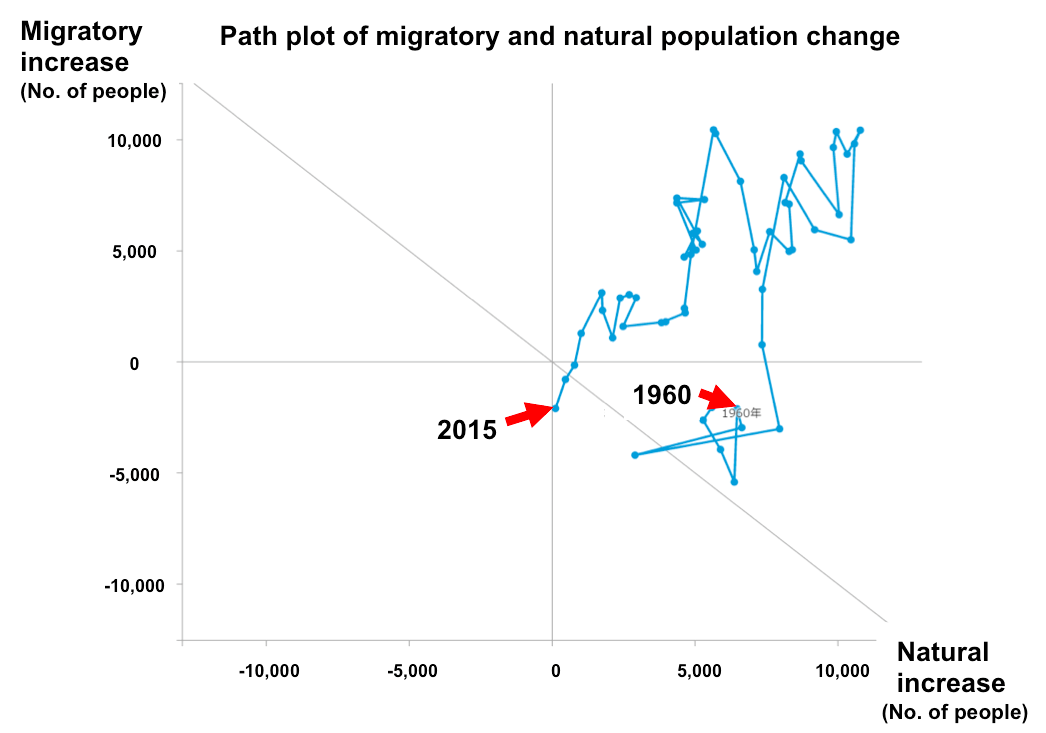
\includegraphics[width= 8cm]{fig/fig2_2.png}
\caption{RESAS path plot of Natural increase ($x$-axis) vs. Migratory increase ($y$-axis) in Shiga. Natural increase equals births minus deaths. Migratory increase equals immigration minus emigration.
\\{\it Data source}: Vital Statistics in Japan, Ministry of Health, Labour and Welfare; Report on Internal Migration in Japan, Ministry of Internal Affairs and Communications.
}\label{fig2}
\end{center}
\end{figure}


\subsection{Population movement}\label{move}

The administrative divisions of Shiga prefecture consist of 13 cities and 6 towns, including the capital city of Otsu.
We summarized migratory statistics for the past three decades at the level of these 19 regions. 
As a result, four cities and one town (Otsu, Hikone, Kusatsu, Moriyama and Aisho) showed migratory increase
---more people entered each city than left the city (Table~\ref{popshiga}). The other 14 regions did not. 

\begin{table}[!t]
\caption{Cities in Shiga having migratory increase during last three decades (avg. per period) }\label{popshiga}
\centering
\begin{tabular}{llrrr}
\hline
\bf City & \bf Number of & \bf 1990s & \bf 2000s & \bf 2010s  \\\hline
Otsu & immigrant & 15140.4 & 13929.3 & 12320.8 \\
 & emigrant & 12980.8 & 12353.7 & 10783.8 \\
 & difference & 2159.6 & 1575.6 & 1537 \\\hline
Hikone & immigrant & 4469.8 & 4452.1 & 4224.8 \\
 & emigrant & 4195.6 & 4357.1 & 3996.8 \\
 & difference & 274.2 & 95 & 228 \\\hline
Kusatsu & immigrant & 7170.4 & 6977.7 & 6960.3\\
 & emigrant & 5634 & 6534.8 & 5816.3 \\
 & difference & 1536.4 & 442.9 & 1144  \\\hline
Moriyama & immigrant & 3067 & 3553.8 & 3325.5 \\ 
 & emigrant & 2716 & 2914.1 & 2940.3 \\ 
 & difference & 351 & 629.7 & 385.3 \\\hline
Aisho$^\dagger$
 & immigrant & 771.2 & 845.2 & 933.5  \\
 & emigrant & 712.6 & 734 & 751  \\
 & difference & 58.6 & 111.2 & 182.6 \\\hline
\multicolumn{5}{l}{$^\dagger$ Aisho is a district of town.}
\\
\multicolumn{5}{l}{{\it Data source}: Report on Internal Migration in Japan, Ministry}
\\
\multicolumn{5}{l}{of Internal Affairs and Communications.}
\\
\end{tabular}
\end{table}


\begin{figure}[!h]
\begin{center}
	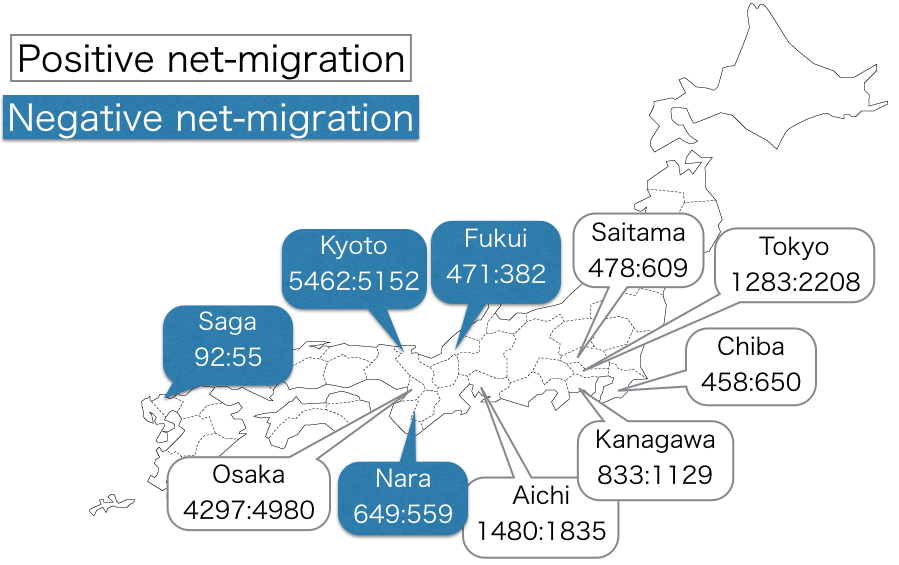
\includegraphics[width= 8cm]{fig/slide.png}
\caption{Prefectures associated to population movement of Shiga prefecture in 2015 (immigrant:emigrant)
\\
{\it Data source}:  Reproduced based on Report on Internal Migration in Japan, Ministry of Internal Affairs and Communications}
\label{fig29}
\end{center}
\end{figure}
\begin{figure}[!t]
\begin{center}
    %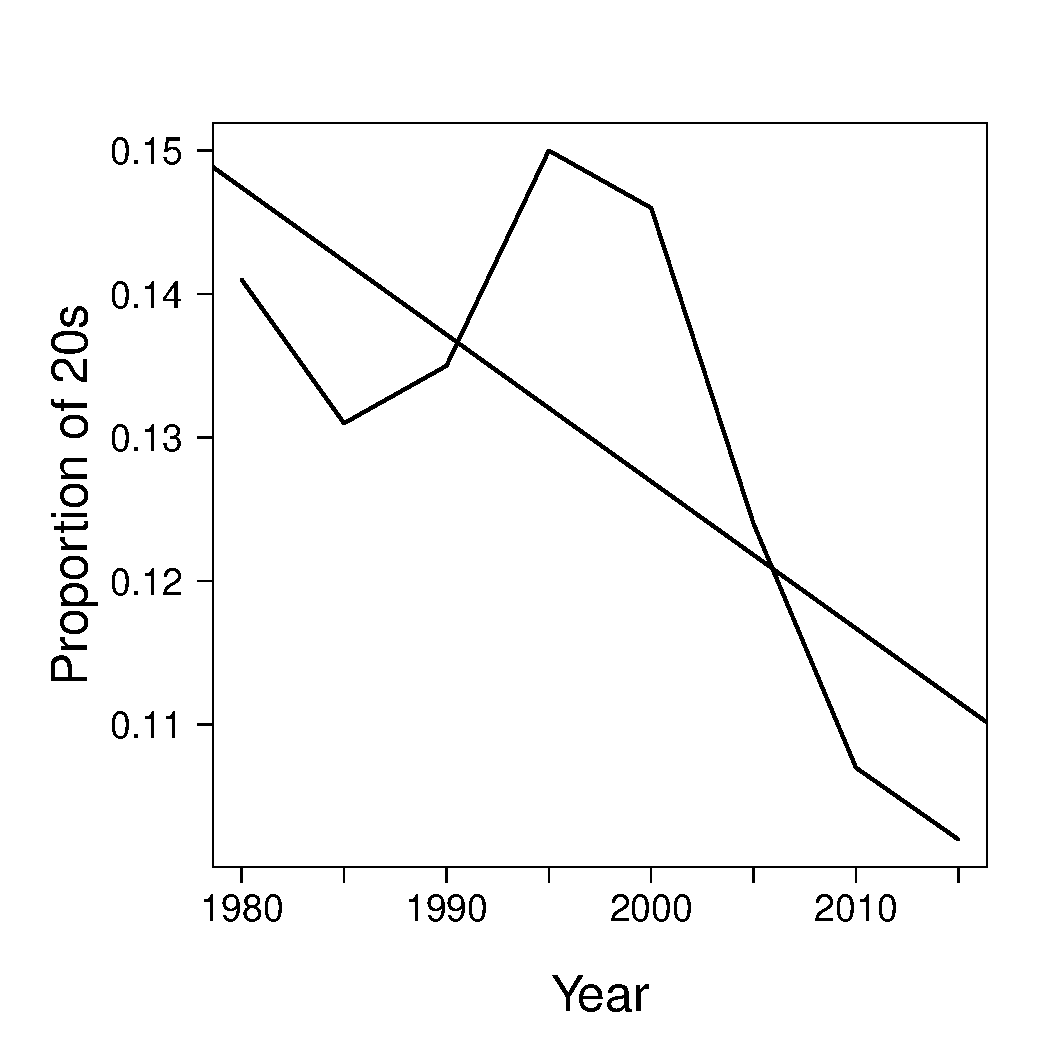
\includegraphics[width= 8cm]{fig/rege2.pdf}
\caption{Linear regression for Proportion of 20s against Year (Otsu city, Shiga). }
\label{fig31}
\end{center}
\end{figure}







Next, we analyzed the population movement between 46 prefectures and Shiga, that is, migration from other prefectures to Shiga or vice versa.
 Fig. \ref{fig29} represents 10 prefectures which gave the statistically significant p-value
of the null hypothesis that
the ratio of immigrant to emigrant is one to one.
For example, there was a statistically significant difference between 5,462 people who moved into Shiga from Kyoto, and 5,152 people who moved out of Shiga to Kyoto.

As seen from Fig.~\ref{fig29}, Tokyo, Chiba, Kanagawa, Aichi, Saitama and Osaka prefectures are the regions with population outflow (more emigration than immigration), while more people moved into Shiga from Saga, Kyoto, Nara and Fukui in 2015. 
This result may be characterized by big city domination. This is due to the migration of labor to major cities, especially the age of 20s, because these cities offer a concentration of business enterprises and
many opportunities for employment.


\subsection{Population change of the age of 20s}\label{reg}
As mentioned in subsection \ref{move}, big city domination is considered as a cause 
for population outflow, especially in the age of 20s. If we consider overall ages, the five regions in Shiga show population increase (Table~\ref{popshiga}).
\begin{figure*}[!t]
\centering
\subfloat[Otsu city (Shiga prefecture)]{
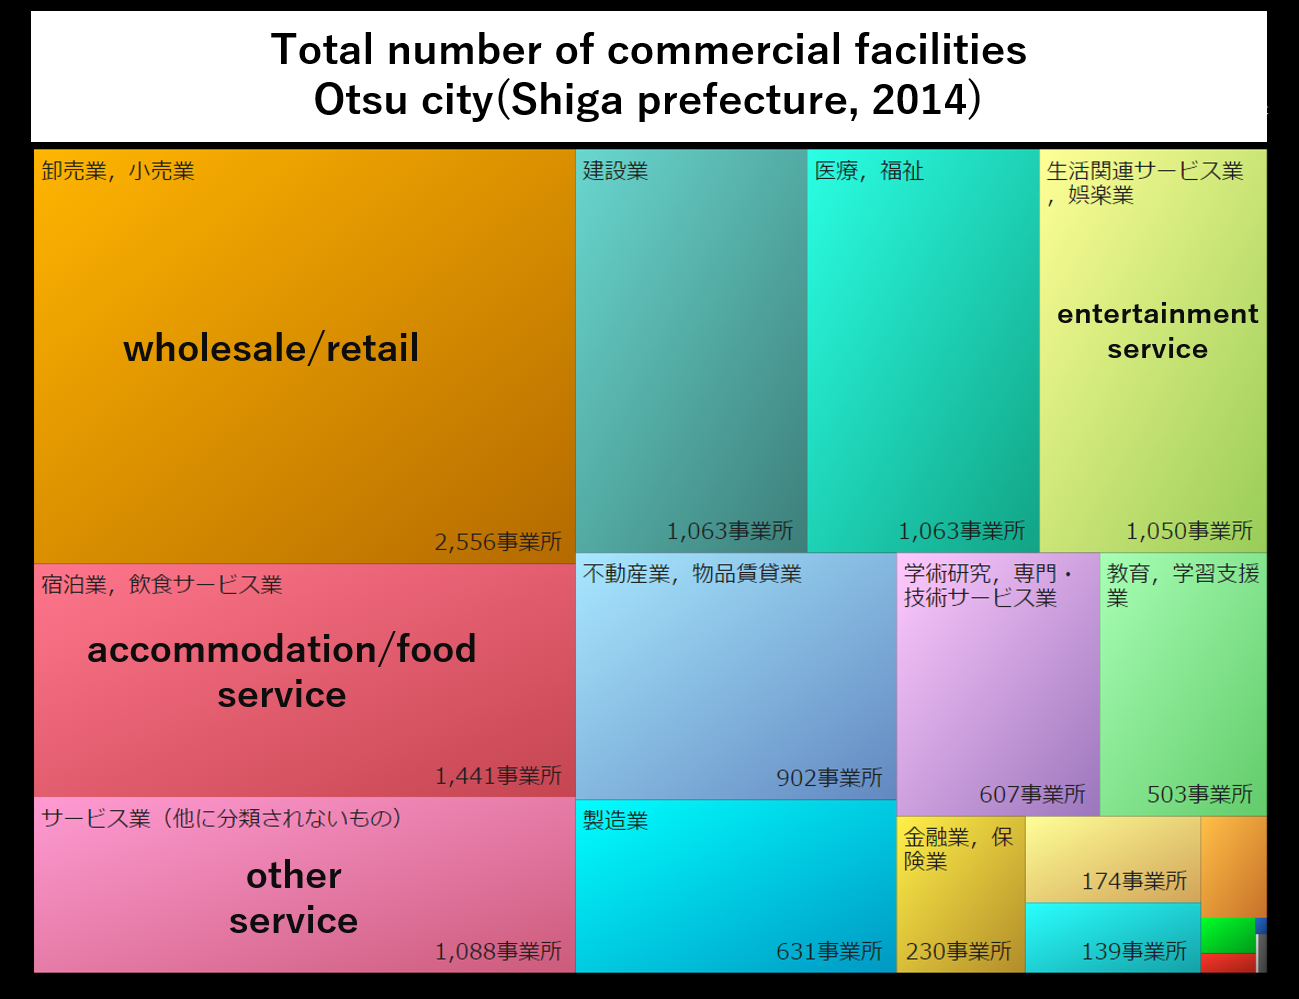
\includegraphics[width= 7cm]{fig/otsu1.png}
}
\qquad
\subfloat[Shisui town (Chiba prefecture)]{
   %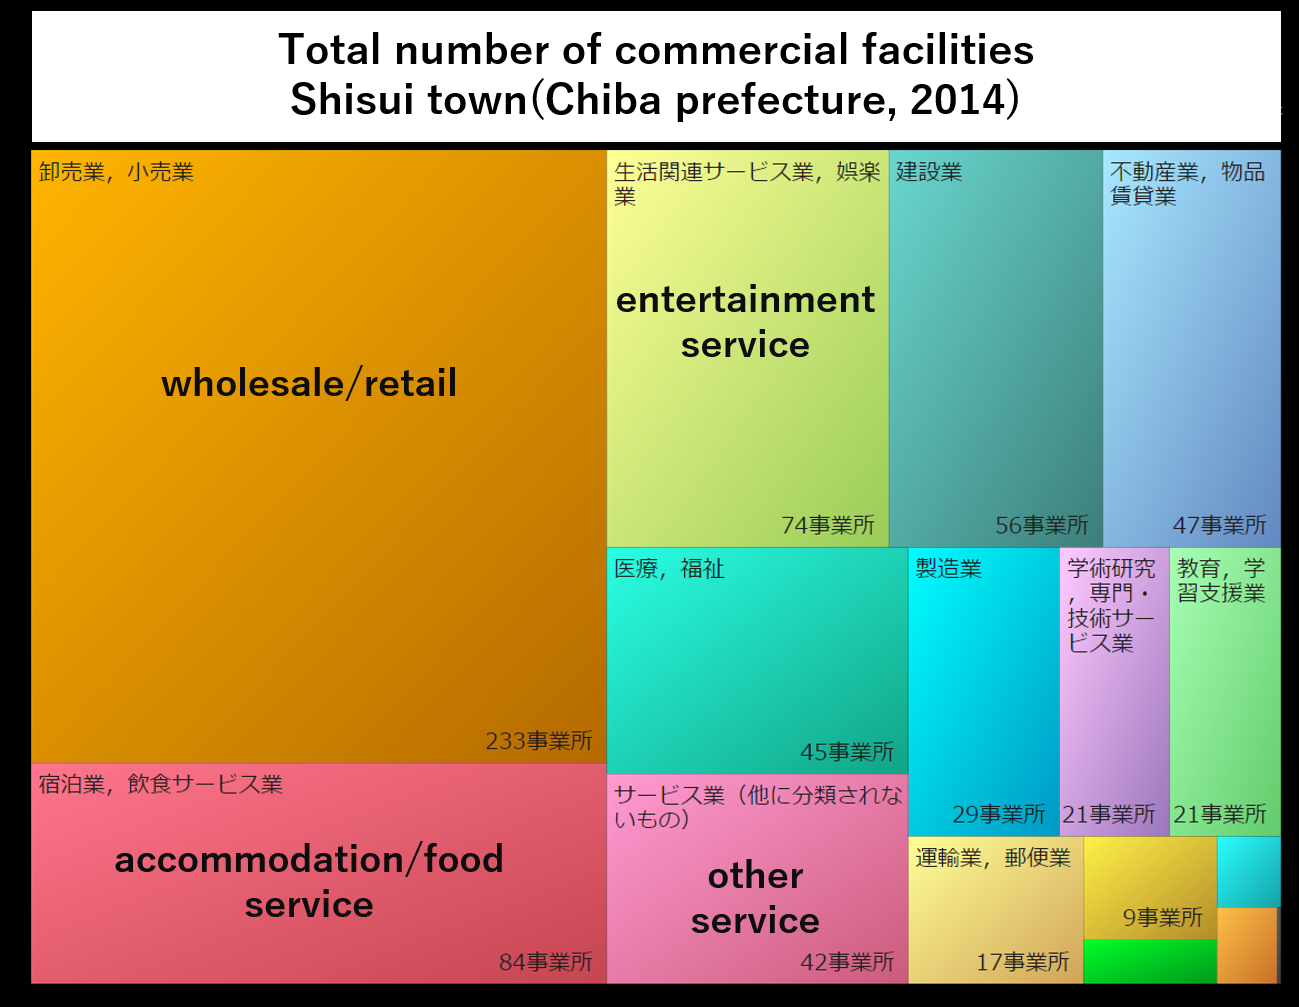
\includegraphics[width= 7cm]{fig/shu1}
}
\caption{RESAS Industrial structure tile plot.
\\{\it Data source}: Economic Census for Business Frame, Ministry of Internal Affairs and Communications;
 Economic Census for Business Activity, Ministry of Economy, Trade and Industry.
}\label{industry}
\end{figure*}


In contrast to overall population increase, the fitted regression line in Fig.~\ref{fig31} suggests that the age of 20s have gradually moved outside Otsu, the capital city of Shiga.
On the contrary, though we do not show regression lines, 
 Shisui town, Sakae town (Chiba prefecture), Ushiku city (Ibaraki prefecture), Ryuo town (Shiga prefecture) and Toyono town (Osaka prefecture) were the regions where the age of 20s are on slightly increasing trend.
 
 \begin{table*}[!t]\caption{Number of arrivals and amount of consumption (2014, avg. per each cluster)}\label{consume}
\centering
\begin{tabular}{lrrrr}
\hline
 &\bf  Domestic &  & \bf Foreign\\
 & \bf arrivals & \bf consumption & \bf arrivals & \bf consumption \\
\bf Cluster & \bf (thousand) & \bf (million yen) & \bf (thousand) & \bf (million yen) \\\hline
Hokkaido,  Shizuoka & 46,185 & \bf{565,948} & \bf{1,295} & \ \mr{168,039} \\
Kanagawa & \bf{93,826} & \bf{690,142} & 521 & \bf{51,862} \\
Saitama, Chiba, Hyogo, Aichi & \bf{84,298} & 436,402 & 210 & 12,705 \\
Osaka & * & * & * & * \\
Fukuoka & * & * & * & * \\
Kyoto, Nara & 37,110 & 243,752 & \bf{780} & 48,773 \\
Tokyo & \mr{234,871} & \mr{1,847,320} & \mr{2,461} & \bf{166,003} \\
Aomori, Akita, Toyama, Ibaraki & 14,904 & 108,354 & 107 & 3,006 \\
Fukui, Tottori, Tokushima, Kagawa, Saga & 12,328 & 133,598 & 60 & 3,498 \\
Iwate,  Miyazaki,  Kagoshima & \mb{11,207} & 117,386 & 92 & 7,224 \\
Ishikawa, Oita, Yamanashi, Mie, Kumamoto, Gifu & 23,442 & 227,539 & 427 & 26,216 \\
Shiga,  Wakayama,  Shimane,  Okayama,  Nagasaki,  Yamaguchi & 12,526 & 117,128 & 133 & 5,411 \\
Hiroshima, Ehime, Kochi & 11,931 & \mb{85,867} & 66 & \mb{2,764} \\
Miyagi,  Gunma,  Yamagata,  Tochigi & 26,598 & 232,044 & \mb{51} & 4,526 \\
Fukushima, Niigata, Nagano & 26,632 & 334,378 & 171 & 12,276 \\
Okinawa & 8,364 & 394, 769 & 502 & 36,969 \\\hline
\multicolumn{5}{l}{The figures in bold red, blue and black indicate maximum, minimum and the second/third respectively.}\\
\multicolumn{5}{l}{Symbol * indicates there is no available data}\\
\multicolumn{5}{l}{{\it Data source}: National Tourism Survey, Consumption Trend Survey for Foreigners Visiting Japan, Japan Tourism Agency.}
\end{tabular}
\end{table*}




\begin{figure*}[!t]
\centering
\begin{center}
   %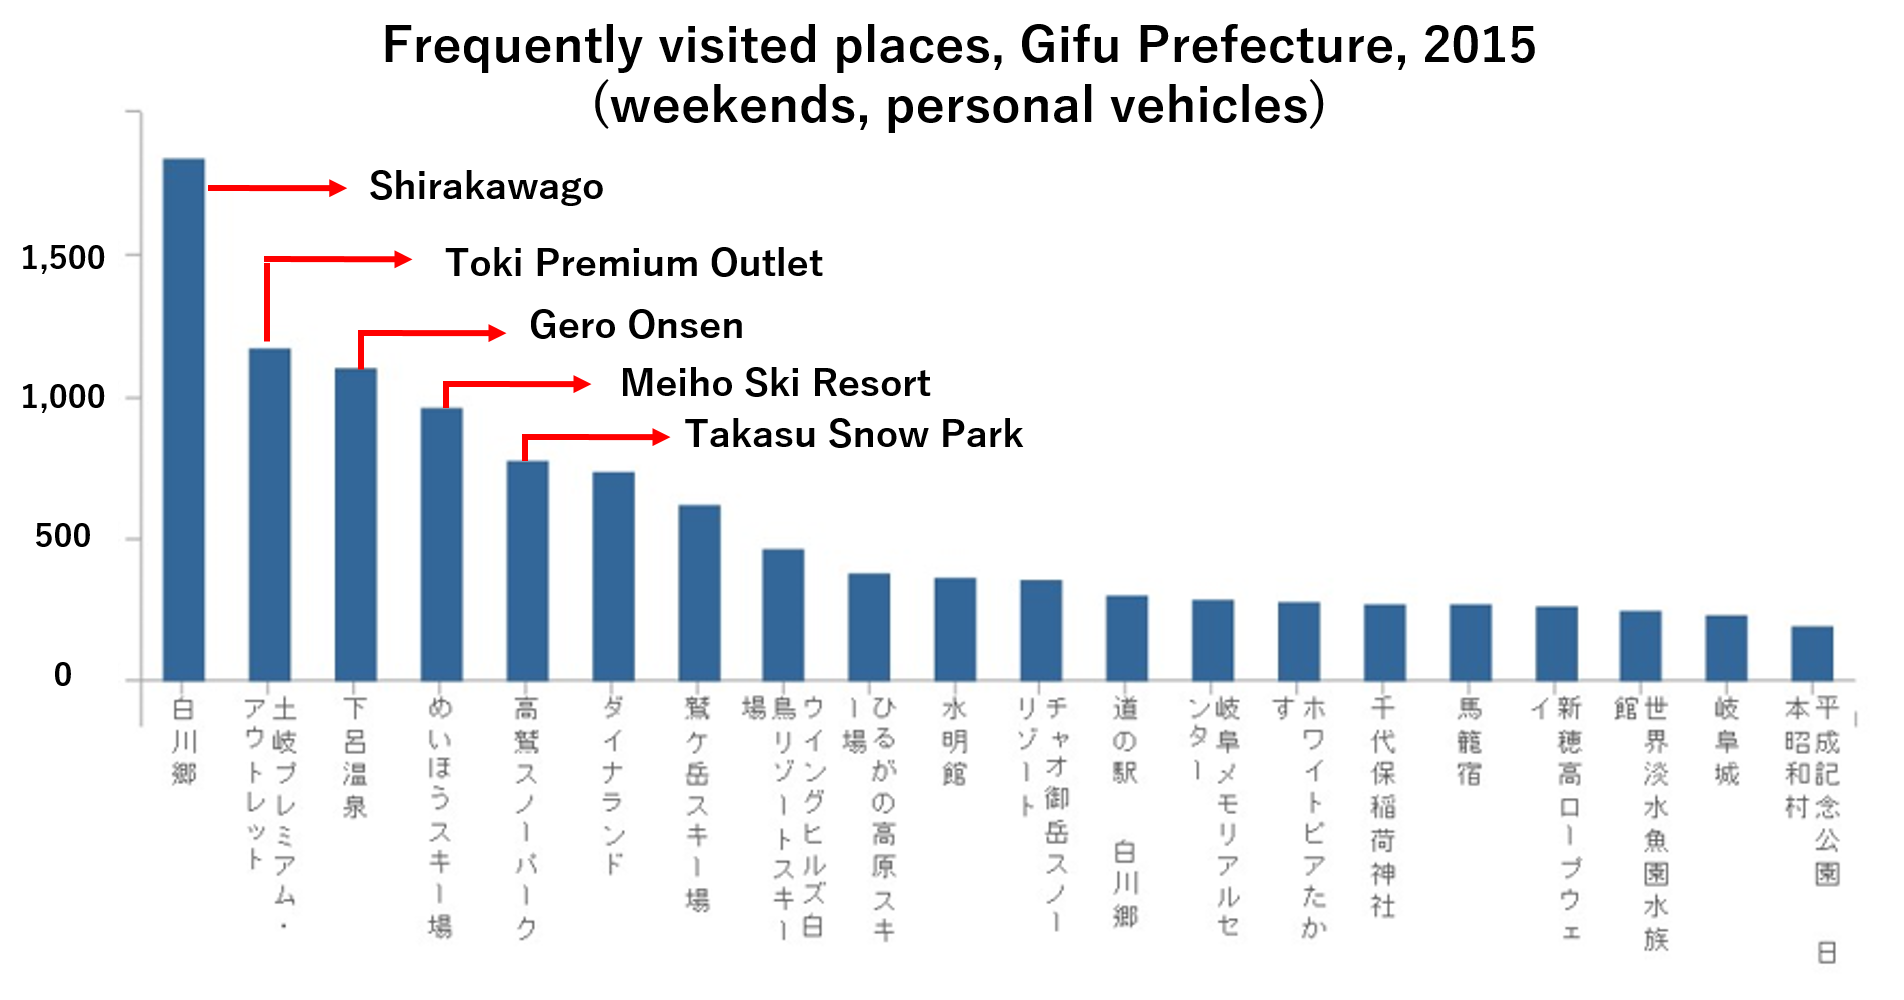
\includegraphics[width= 13cm]{fig/fig3_1}
\caption{RESAS destination searching (weekends, personal vehicles). Frequently visited places of Gifu in 2015.
\\{\it Data source}: NAVITIME JAPAN Co.
}\label{gifu1}
\end{center}
\end{figure*}

One of the reasons for their behavior could be due to the industrial structure. 
To clarify the difference between Otsu and these five cities, we used industrial structure menu in RESAS.
Fig. \ref{industry} illustrates the results of Otsu city and Shisui town.
Orange, red and pink color tile in Fig. \ref{industry} represents wholesale/retail, accommodation/food and other service, respectively. The other kinds of facility of medical/welfare, real estates, research, manufacture, etc. are represented by other colors.

Among the six regions, Otsu has shown that it has less commercial facilities related to wholesale/retail and accommodation/food than those of others. This suggests that population change of age of 20s is correlated with industries of wholesale/retail and accommodation/food. We recommend that local government of Shiga should consider industrial structure when planning population policy for age of 20s.
%----------------------------------------------------------------

\section{Tourism in Shiga}\label{sec:tour}
This section introduces a different approach to Shiga from tourism point of view, including the topics on domestic or international tourism consumption, number of tourists and attractiveness of Shiga. 
In a similar way to the previous section, tourism data were gathered from the government websites. 

\subsection{Clustering 47 prefectures}\label{clus}


We divided 47 prefectures into several groups by cluster analysis, using the tourism variables summarized in Table~\ref{data}, so that prefectures in the same group are more similar to each other than to those in other groups.
Table~\ref{consume} shows each cluster's summary statistics of tourist arrivals and consumption. 



\begin{table}[!h]\caption{Variables related to tourism}\label{data}
\centering
\begin{tabular}{l|l|l}
\hline
\bf Category & \bf Variable & \bf Unit \\\hline
Location & distance from the major city& km \\\hline
Nature & nature conservation area &ha\\\hline
Economy & prefecture GDP & million yen\\
 & population & \\
 & area / person& $m^2$\\\hline
Cultural Properties & National Treasures &  \\
 & Important Cultural Property  &  \\
 & Special heritage, etc.  \\\hline
Entertainment & Leisure facilities \\\hline
Tourism infrastructure & Hotel \\
 & Ryokan  \\\hline
Tourist arrivals & & thousand\\
Tourist consumption &  & million yen \\\hline %\llap
\end{tabular}
\end{table}
\begin{table*}[!t]\caption{Number of tourists and amount of consumption in 2014}
\label{kanko}
\centering
\begin{tabular}{r|rrr|rrr}
\hline
 & \bf Shiga cluster &  &  & \bf Target cluster &  &  \\
 & \bf Prefecture & \bf Tourists & \bf Consumption & \bf Prefecture & \bf Tourists & \bf Consumption \\
 & & \bf (thousand) & \bf (million yen) & & \bf (thousand) & \bf (million yen) \\\hline
Domestic & \bf{Shiga} & \bf16,030 & \bf124,394 & Ishikawa & 14,948 & 189,681 \\
 & Wakayama & 9,516 & 120,481 & Oita & 16,412 & 143,185 \\
 & Shimane & 10,595 & 72,739 & \bf{Yamanashi} & \bf26,470 & \bf299,845 \\
 & Okayama & 10,356 & 103,527 & Mie & 27,211 & 264,262 \\
 & Nagasaki & 2,614 & 72,263 & Kumamoto & 21,625 & 267,226 \\
 & Yamaguchi & 15,277 & 108,302 & \bf{\bf{Gifu}} & \bf{33,983} & \bf201,034 \\ \hline
Foreign & \bf{Shiga} & \bf138 & \bf 8,381 & Ishikawa & 149 & 10,086 \\
 & Wakayama & 178 & 11,680 & Oita & 327 & 5,106 \\
 & Shimane & 37 & 1,513 & \bf{Yamanashi} & \bf{1,162} & \bf 103,428 \\
 & Okayama & 57 & 1,806 & Mie & 82 & 4,895 \\
 & Nagasaki & 368 & 8,208 & Kumamoto & 341 & 6,119 \\
 & Yamaguchi & 22 & 875 & \bf{Gifu} & \bf500 & \bf27,660 \\\hline
\multicolumn{7}{l}{{\it Data source}: National Tourism Survey, Consumption Trend Survey for Foreigners Visiting Japan, Japan Tourism Agency.}
\end{tabular}
\end{table*}

Shiga prefecture was assigned to the cluster consisting of Shiga, Wakayama, Shimane, Okayama, Nagasaki and Yamaguchi. 
The second similar cluster to Shiga is the cluster of Ishikawa, Oita, Yamanashi, Mie, Kumamoto and Gifu, which show two to five times more arrivals and consumption both domestic and international.
For this reason, we refer to the former as ``Shiga cluster" and to the latter as ``target cluster". 


 \begin{table}[!h]\caption{Destinations of Gifu and Yamanashi ranked in top 5}
\label{dest}
%\tiny
\centering
\begin{tabular}{rll}
\hline
 & \bf Personal Vehicles& \bf Public Transportation \\ \hline
\bf Rank & \bf Gifu Prefecture \\\hline
1 & Shirakawago & Shirakawago \\
2 & Toki Premium Outlet & Gero Onsen \\
3 & Gero Onsen & Toki Premium Outlet \\
4 & Meiho Ski Resort & Dyno Land \\
%5 & ​​Takasu Snow Park & ​​Meiho Ski Resort \\ \hline
\bf  Rank & \bf Yamanashi Prefecture \\\hline
1 & Fujiten Resort & Fujikyu Highland \\
2 & Lake Kawaguchi & Lake Yamanaka \\
3 & Lake Yamanaka & Lake Kawaguchi \\
4 & Fujikyu Highland & Hottarakashi Onsen\\
%5 & ​​Kamuimisaka Ski Resort & Fujiten Snow Resort \\
\hline
\multicolumn{3}{l}{{\it Data source}: NAVITIME JAPAN Co.}
\end{tabular}
\end{table}

\begin{figure*}[!t]
\centering
\subfloat[MDS of distance matrix]{
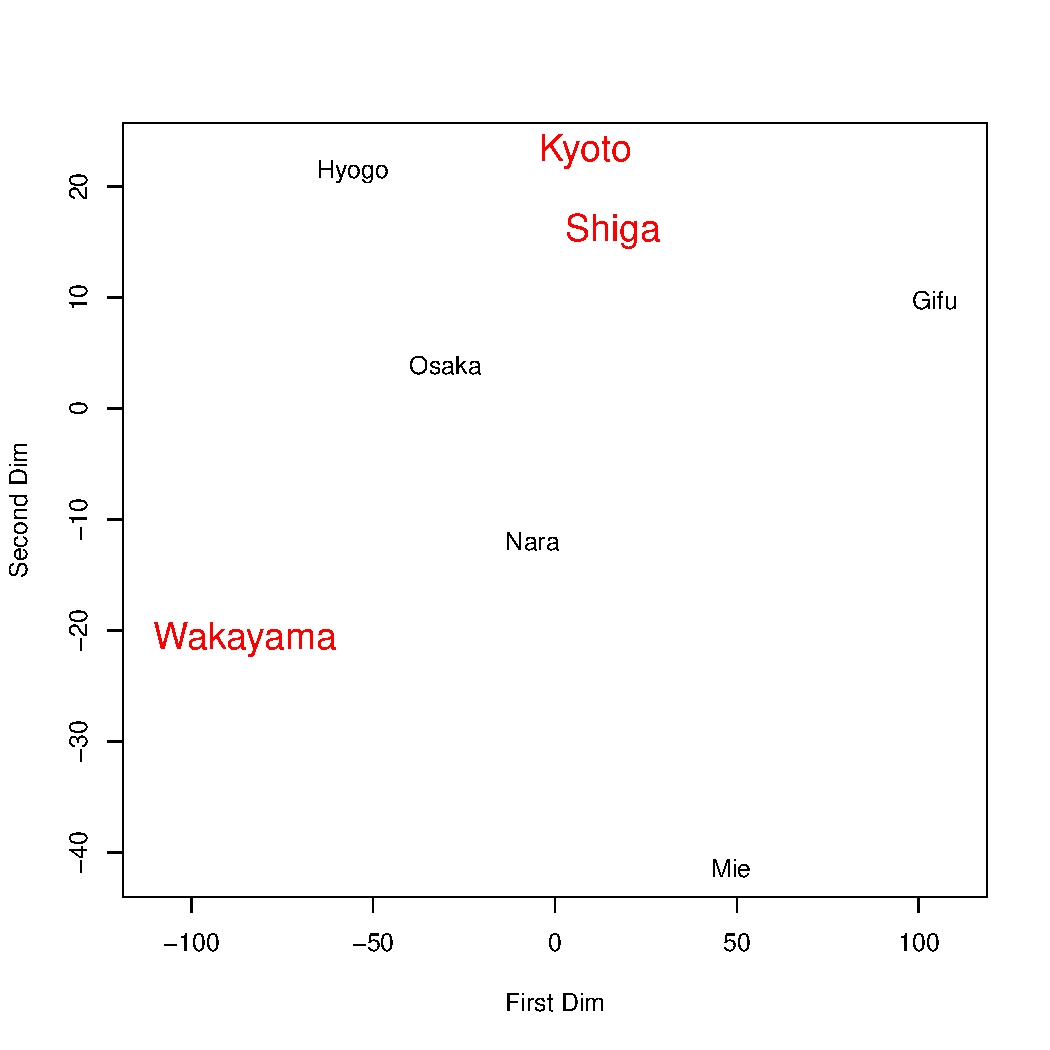
\includegraphics[width= 7cm]{fig/mds1e.pdf}
}
\qquad
\subfloat[MDS of tourism resources]{
   %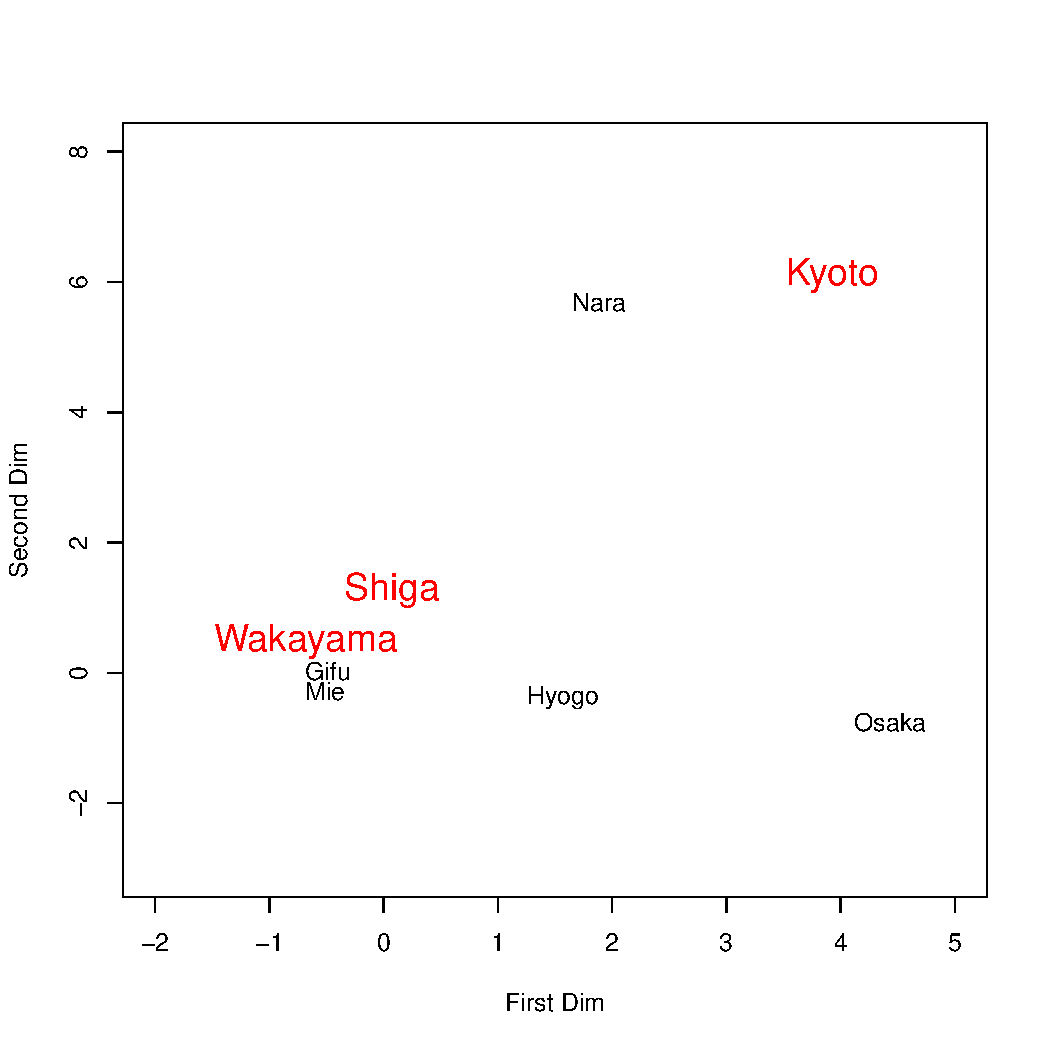
\includegraphics[width= 7cm]{fig/mdse.pdf}
}
\caption{Multidimensional scaling (MDS) with variables of geographical distance and tourism resources of 47 prefectures. Prefectures which are not included in Table \ref{percent} were masked.
\\{\it Data source}: Geospatial Information Authority of Japan(www.gsi.go.jp/KOKUJYOHO/kenchokan.html).}\label{multi}
\end{figure*}




Further investigation of target cluster showed that Gifu and Yamanashi are the most popular  prefectures in terms of domestic tourist arrivals and international tourist arrivals, respectively (Table~\ref{kanko}).
We will discuss more details about these two prefectures, in the next subsection.


\subsection{Searching destination}

Although there are some limitations, RESAS provides quite good visualizations of some private commercial data as well as public data. For example, RESAS's destination menu gives frequently searched destination rankings through car navigations data, which is offered by NAVITIME JAPAN Co. Fig.~\ref{gifu1} illustrates Gifu's frequently searched destinations, by retrieving under the condition of weekends and personal vehicles in 2015. 


We retrieved in the same manner the most visited places in Gifu and Yamanashi by personal vehicles or public transportation.
As can be seen from Table~\ref{dest}, 
both prefectures are characterized by World Heritage, ski resorts and onsen (hot spring). 

It should also be noted that Shiga already has these tourism factors such as, 
World Heritage of Hieizan Enryakuji, ski resort of Biwako Valley and hot spring Ogoto Onsen.
Nevertheless, the amount of consumption and number of tourists in Shiga, shown in Table~\ref{kanko}, are far below those of Yamanashi and Gifu.


\subsection{Accessibility to Kyoto}


Kyoto is one of the world's most popular cities to visit and Shiga has a good advantage of accessibility to Kyoto as well as its own tourism resources mentioned above.
However, among more than four million foreign tourists visiting Japan in 2015, only about 2\% (eighty thousand) visited Shiga (Table \ref{percent}).

\begin{table}[!h]\caption{Total number of foreign arrivals in Kyoto prefecture and adjacent prefecture, 2015}
\label{percent}
\centering
\begin{tabular}{l|r|rrr}
\hline
\bf Prefecture & \bf Kyoto  & \bf Gifu  & \bf Mie  & \bf Shiga  \\\hline
No. of arrivals & 4,165,875 & 437,506 & 60,640 & 80,211\\
\% & - & 10.50\% & 1.46\% & 1.93\% \\\hline
\bf Prefecture & \bf Kyoto & \bf Hyogo  & \bf Nara  & \bf Wakayama  \\\hline
No. of arrivals & 4,165,875 & 1,007,093 & 900,455 & 197,589 \\
\% & - & 24.17\% & 21.62\% & 4.74\% \\\hline
\multicolumn{5}{l}{{\it Data source}: Consumption Trend Survey for Foreigners Visiting}\\
\multicolumn{5}{l}{Japan, Japan Tourism Agency.}
\end{tabular}
\end{table}

The question here arises: Dose Shiga make a good use of its locational advantage?
To answer this question, it is worthwhile comparing Wakayama and Shiga prefectures, 
because these are the closest to Kyoto among the 
prefectures in Shiga cluster (which is defined in section \ref{clus}). 


Fig. \ref{multi} shows multidimensional scaling (MDS) plots with variables of geographical distance and tourism resources, respectively.
In terms of tourism resources, Kyoto is relatively closer to Shiga than Wakayama, as is the case of geographical distance. As seen from Table~\ref{kanko}, there are more domestic tourists in Shiga than Wakayama,
which implies that the short distance between Shiga and Kyoto seems to 
result in the increase of domestic tourists.
However, that is not the case in foreign tourists; that is, 
fewer number of foreign tourists visited Shiga than Wakayama.

The above results suggest that local government of Shiga does not make full use of its geographical advantage. 
Therefore, when planning a tourism strategy for foreign countries, 
it should be addressed that Shiga is not only attractive but also convenient to access from Kyoto. 

\section{Discussion}\label{sec:discuss}
In this paper, we discussed topics concerning population and tourism of Shiga prefecture by using government open data, RESAS and several traditional statistical analyses. 

As a result, we realized again the overall decline of population in Shiga, but five cities (Otsu, Hikone, Kusatsu, Moriyama and Aisho) have been found to be in increasing trends. Saga, Kyoto, Nara and Fukui prefectures seemed to be highly related to Shiga's population change. Shisui town, Ushiku city, Ryuo town, Toyono town and Sakae town are the regions in which the age of 20s are slightly increasing. 
For the tourism analysis, we have found that Yamanashi and Gifu prefecture might be target prefectures of Shiga based on tourism GOD. We also derived three key words of World Heritage, ski resorts and onsen.  
Our research suggests that the policy makers of local government of Shiga should take into consideration the results above, when planning regional economy policy.


Finally, we discuss several limitations of our study and RESAS.
First, although RESAS is equipped with useful visualization tools concerning various topics such as regional economics, industrial structure, business company, employment, comparison among the prefectures, etc., we have used only population and tourism menus to visualize Shiga. Second, in population analysis of section \ref{reg}, we adopted simple regression model with time variable as explanatory variable on proportion of age of 20s, but it is worth considering other explanatory variables such as birth rate.
Third, RESAS is a well-organized tool, especially for beginners, to  visualize regional economy, but it still dose not allow to export the graph shown on the screen. Fourth, at the present moment, RESAS provides results only in Japanese language, so the RESAS graphs and results which are presented in this paper were partly edited manually to be shown in English.

Despite the limitation of our study, we hope that these results will give an idea of how to analyze regional social problems by using GOD, RESAS and statistical analysis.

\bibliography{zzz}
\end{document}


